\ifdefined\COMPILINGFROMMAIN
\else
    %%%%HEADER
\documentclass[twocolumn]{article}
\usepackage[a4paper, margin=1in, columnsep=20pt]{geometry}
\usepackage{amsmath, amssymb, graphicx, hyperref}
\usepackage[most,skins,breakable]{tcolorbox}
\usepackage[symbol]{footmisc}
\usetikzlibrary{calc}
\usepackage{xcolor}
\usepackage{caption}
\usepackage{algorithm}
\usepackage{algpseudocodex}
\usepackage{tikz}
\usepackage{listings}
\usetikzlibrary{arrows.meta, positioning}
\tcbuselibrary{listingsutf8}
\usepackage{microtype}
\usepackage{blindtext}
\usepackage{bookmark}
\usepackage{breqn}
\usepackage[backend=biber,style=numeric]{biblatex} % 
\addbibresource{../references.bib}

% Define style for the listings environment
\lstdefinestyle{mystyle}{
    basicstyle=\ttfamily\small,
    breaklines=true,
    escapeinside={(*@}{@*)}, % Allows math mode within listings
    numbers=left,
    numberstyle=\tiny,
    frame=single,
    keywordstyle=\color{blue}\bfseries,
    commentstyle=\color{green!50!black},
    stringstyle=\color{red}
}


\def\reals{\mathbb{R}}
% Define the custom definition box and command
\newtcolorbox{mydefinition}[2][]{%
    text width=0.95\columnwidth,
    before=\vspace{1mm}, 
    after=\vspace{1mm}, 
    colback=gray!10, % Background color (light gray)
    colframe=black!70,  % Border color
    coltitle=gray!10,  % Title color
    fonttitle=\bfseries, % Title font style
    sharp corners,   % Box style
    left=2pt,
    breakable,
    right=2pt,
    top=2pt,
    bottom=2pt,
    enhanced jigsaw,
    title=Definition: {#1},         % Title passed as the first argument
    colupper=black,  % Ensure proper content handling
    pad at break*=1pc,
    overlay first and middle={
        \coordinate (A1) at ($(interior.south east) + (-10pt,5pt)$);
        \coordinate (C1) at ($(interior.south east) + (-6pt,7.5pt)$);
        \draw[fill=black!50] (A1) -- +(0,5pt) -- (C1) -- cycle;
    }
    }
    
\newcommand{\definition}[2]{%
    \noindent%
    \begin{mydefinition}[#1]%
        .#2%
    \end{mydefinition}%
    \noindent
}

\newtcolorbox{myexample}[2][]{%
    text width=0.95\columnwidth,
    before=\vspace{1mm}, 
    after=\vspace{1mm}, 
    colback=orange!3, % Background color (light gray)
    colframe=black!70,  % Border color
    coltitle=gray!10,  % Title color
    fonttitle=\bfseries, % Title font style
    sharp corners,   % Box style
    left=2pt,
    right=2pt,
    top=2pt,
    bottom=2pt,
    breakable,
    title=Intuition: {#1},         % Title passed as the first argument
    pad at break*=1pc,
    overlay first and middle={
        \coordinate (A1) at ($(interior.south east) + (-10pt,5pt)$);
        \coordinate (C1) at ($(interior.south east) + (-6pt,7.5pt)$);
        \draw[fill=black!50] (A1) -- +(0,5pt) -- (C1) -- cycle;
    }
}

\newcommand{\example}[2]{%
    \noindent%
    \begin{myexample}[#1]%
    .#2%
    \end{myexample}%
    \noindent
}

\newtcolorbox{algobox}[2][]{%
    text width=0.95\columnwidth,
    before=\vspace{1mm}, 
    after=\vspace{1mm}, 
    colback=blue!5, % Background color (light gray)
    colframe=black!70,  % Border color
    coltitle=gray!10,  % Title color
    fonttitle=\bfseries, % Title font style
    sharp corners,   % Box style
    left=2pt,
    right=2pt,
    top=2pt,
    bottom=2pt,
    breakable,
    title=Algorithm: {#1},         % Title passed as the first argument
    pad at break*=1pc,
    overlay first and middle={
        \coordinate (A1) at ($(interior.south east) + (-10pt,5pt)$);
        \coordinate (C1) at ($(interior.south east) + (-6pt,7.5pt)$);
        \draw[fill=black!50] (A1) -- +(0,5pt) -- (C1) -- cycle;
    }
}

\newcommand{\algorithmbox}[2]{%
\noindent%
    \begin{algobox}[#1]%
    .#2%
    \end{algobox}%
    \noindent
}
%%%%HEADER

    \begin{document}
\fi


\section*{Probabilistic Numerical Solvers for ODEs}
A probabilistic numerical (PN) solver of ODEs is fundamentally different than a classic numerical solver.
A PN starts with a prior distribution over solutions of the solution function $u$, which is then conditioned on information about the vector field $f$. The resulting posterior distribution is referred to as a PN solution of the ODE \cite{nicoThesis}.
We will go through the different steps and cover the prerequisites.

\subsection*{Specifying a Prior Distribution}
Prior distributions over functions are a natural way to model uncertainty in the solution of an ODE. We are interested in tractable computation of the later posterior, which limits our choice of prior. Our prior distribution should be a distribution over functions that is easy to sample from and easy to condition on information. We will focus on the class of Gauss-Markov (\cite{gp_Rasmussen}) processes, which are a Gaussian processes that additionally have the Markov property.
\definition{Markov Property}{
    A stochastic process $U$ has the Markov property if for all $i < s < t$ $$U(t) \perp U(i) \;|\; U(s)$$
    In words, the future is independent of the past given the present. The state at time $t$ must therefore contain all relevant information about the past.
}
In particular, we will use a Gauss-Markov prior for the full state-space representation of $u$, containing $u$ and its first $q\geq 1$ time-derivatives. 
$$\vec{U} :=\begin{bmatrix} U & \frac{d}{d t} U & \cdots & \frac{d^q}{d t^q} U\end{bmatrix}^{\top} \sim \mathcal{GP}$$

\subsubsection*{Linear Time-Invariant Stochastic Differential Equation}
Linear TI SDEs are a class of SDEs that are linear in the state and the noise, and whose system matrices do not depend on the current time.
\definition{Linear Time-Invariant Stochastic Differential Equation}{
    A linear SDE can be written in the form
    \begin{align}\label{eq:LSDE_definition}
        dX(t) = F X(t) dt + L dW(t)
    \end{align}
    where $X(t)\in \reals^n$ is the state, $F\in \reals^{n \times n}$ is the system matrix, $L\in \reals^{n \times n}$ is the diffusion matrix, and $W(t)\in \reals^n$ is a Wiener process. This is known as the Itô form of the SDE. The solution of the SDE is a stochastic process $X(t)$ (\cite{sde-book}).
}
They are a simple choice for the dynamics of the state-space representation of the solution function $u$ and have closed form solutions for the posterior distribution.
\example{Motivating Linear SDEs}{
    A linear SDE can be obtained by injecting gaussian noise into a deterministic ODE. If we start off with the harmonic oscillator with an external force $f(t)$
    $$\frac{d^2}{dt^2}u = -ku - l\frac{d}{dt}u + f(t)$$
    If we do not know the external force and believe it to be independent of previous terms, we might model it as a gaussian noise term $\xi(t) \sim \mathcal{N}(0, \sigma^2)$, giving the linear SDE
    $$\frac{d^2}{dt^2}U = -kU - l\frac{d}{dt}U + \xi(t)$$
    This states that the second derivative is a combination of the first derivative and the function itself, plus noise. The noise makes the system stochastic, hence the capital $U$ notation. TODO SUS However, the noise is nowhere differentiable, and so the expression $\frac{d^2}{dt^2}U$ is not defined. We avoid this issue by combining the SDE notation with a state-space representation of $U$ as $\vec{U} = [U \; \frac{d}{dt}U]^\top$
    $$d\vec{U} = \begin{bmatrix} 0 & 1 \\ -k & -l \end{bmatrix} \vec{U} dt + \begin{bmatrix} 0 & 0 \\ 0 & \sigma \end{bmatrix} dW(t)$$
    Below is shown this spring model. The initial distribution of the state is chosen as $$\vec{U}(0) \sim \mathcal{N}([1, 0]^\top, \text{diag}([0.2^2, 0.1^2]))$$
    \begin{center}
        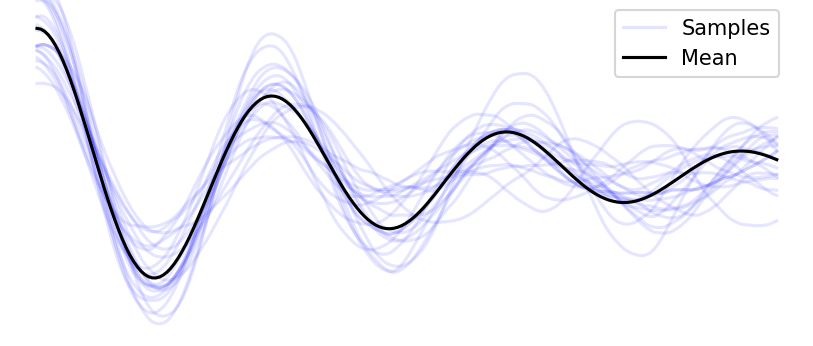
\includegraphics[width=\columnwidth]{../images/stochastic_spring_samples.png}
        \captionof{figure}{50 samples from the linear SDE describing the stochastic spring model with random independent force. The random force has $\sigma = 0.1$ and we have $k=1$, $l=0.2$.}
    \end{center}
}
\newpage
\definition{Integrated Wiener Process}{
    \begin{center}
        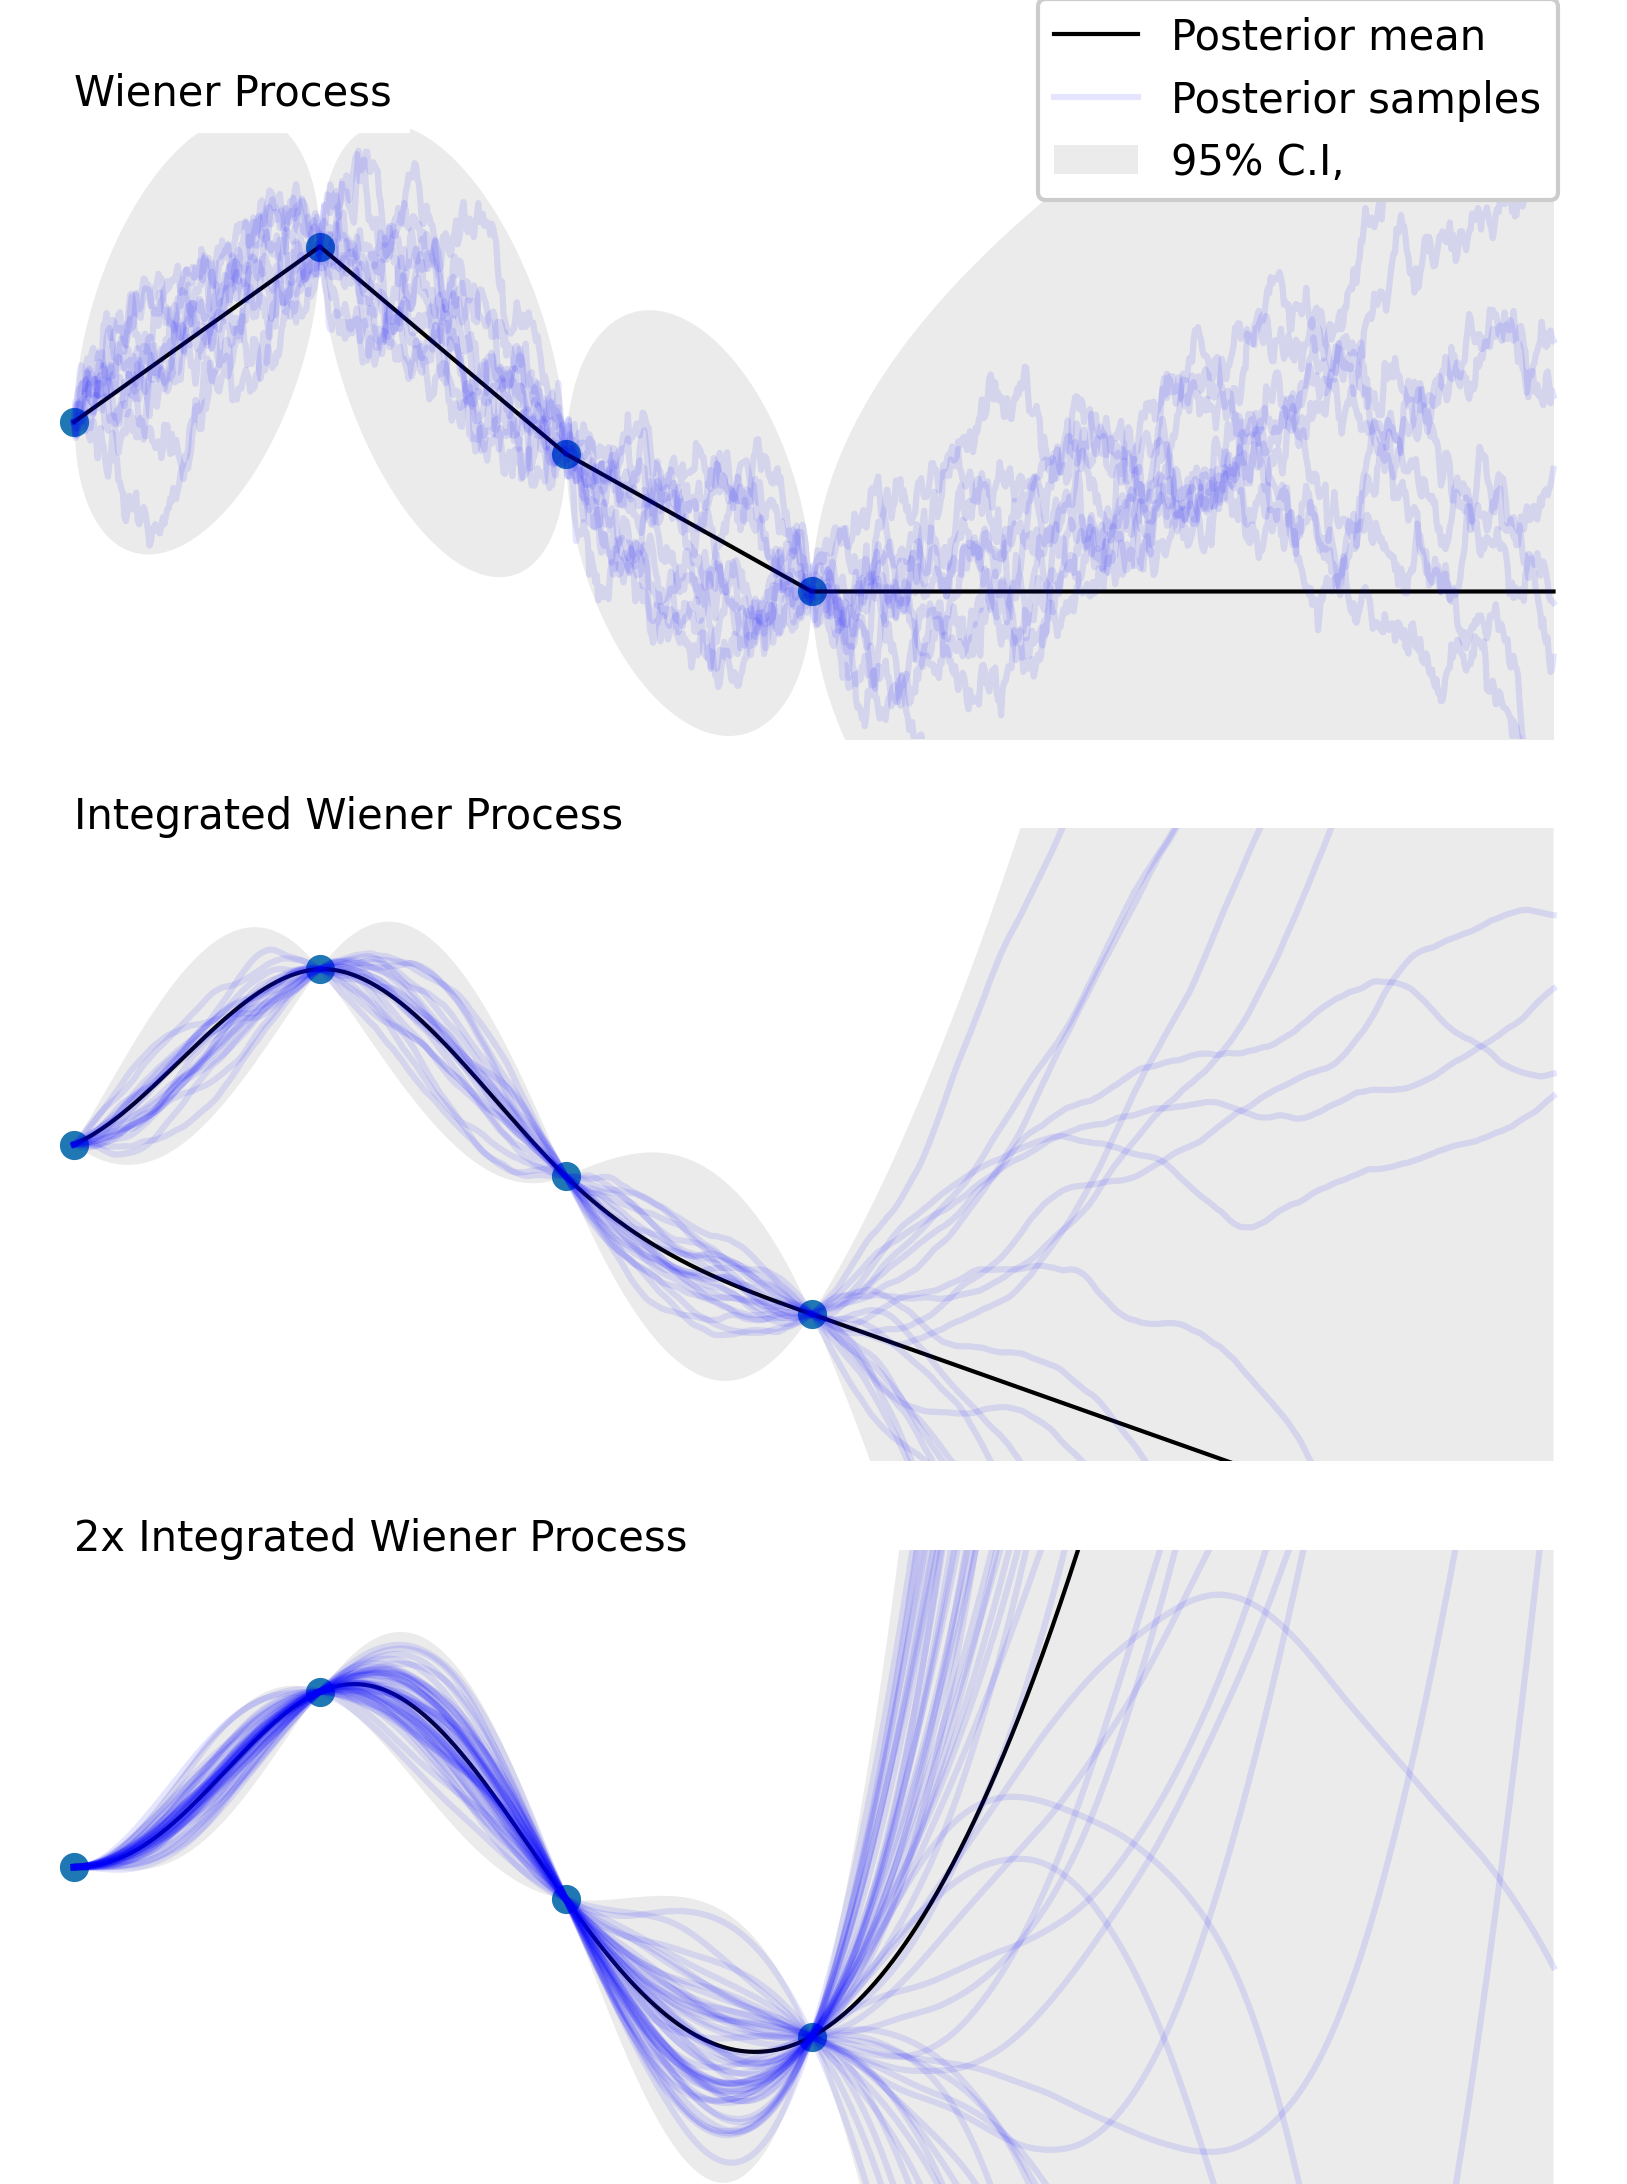
\includegraphics[width=\columnwidth]{../images/conditioned_iwps.png}
        \captionof{figure}{Three graphs of the [x-Integrated] Wiener Process. The processes are conditioned to pass through four different points, marked in blue, the derivative is however unspecified.}
        \label{fig:iwps}
    \end{center}
    The Wiener Process, also known as Brownian motion, is continuous but nowhere differentiable. In terms of eq. \ref{eq:LSDE_definition} its state-space representation is 1-dimensional with $$F=0  \hspace{1cm}L=1$$ 
    The Integrated Wiener Process is the integral of the Wiener Process. The state-space representation is 2-dimensional with $$F=\begin{bmatrix}
        0 & 1 \\ 0 & 0
    \end{bmatrix} \hspace{1cm} L=\begin{bmatrix}
        0 & 0 \\ 
        0 & 1 
    \end{bmatrix}$$
    \\ The Twice Integrated Wiener Process has 3-dimensional state-space with $$F=\begin{bmatrix}
        0 & 1 & 0 \\ 0 & 0 & 1 \\ 0 & 0 & 0
    \end{bmatrix} \hspace{1cm} L=\begin{bmatrix}
        0 & 0 & 0 \\ 0 & 0 & 0 \\ 0 & 0 & 1
    \end{bmatrix}$$
    \\ The posterior means of the $q$-times integrated Wiener process are 2q + 1-ic splines (\cite{probnum}) - see the figure above. There is in principle nothing preventing us from using higher order integrated Wiener processes, but numerical issues are encountered at around $q=3$. We will tackle this later.
}
\newpage
\definition{Ornstein Uhlenbeck Process}{
    \begin{center}
        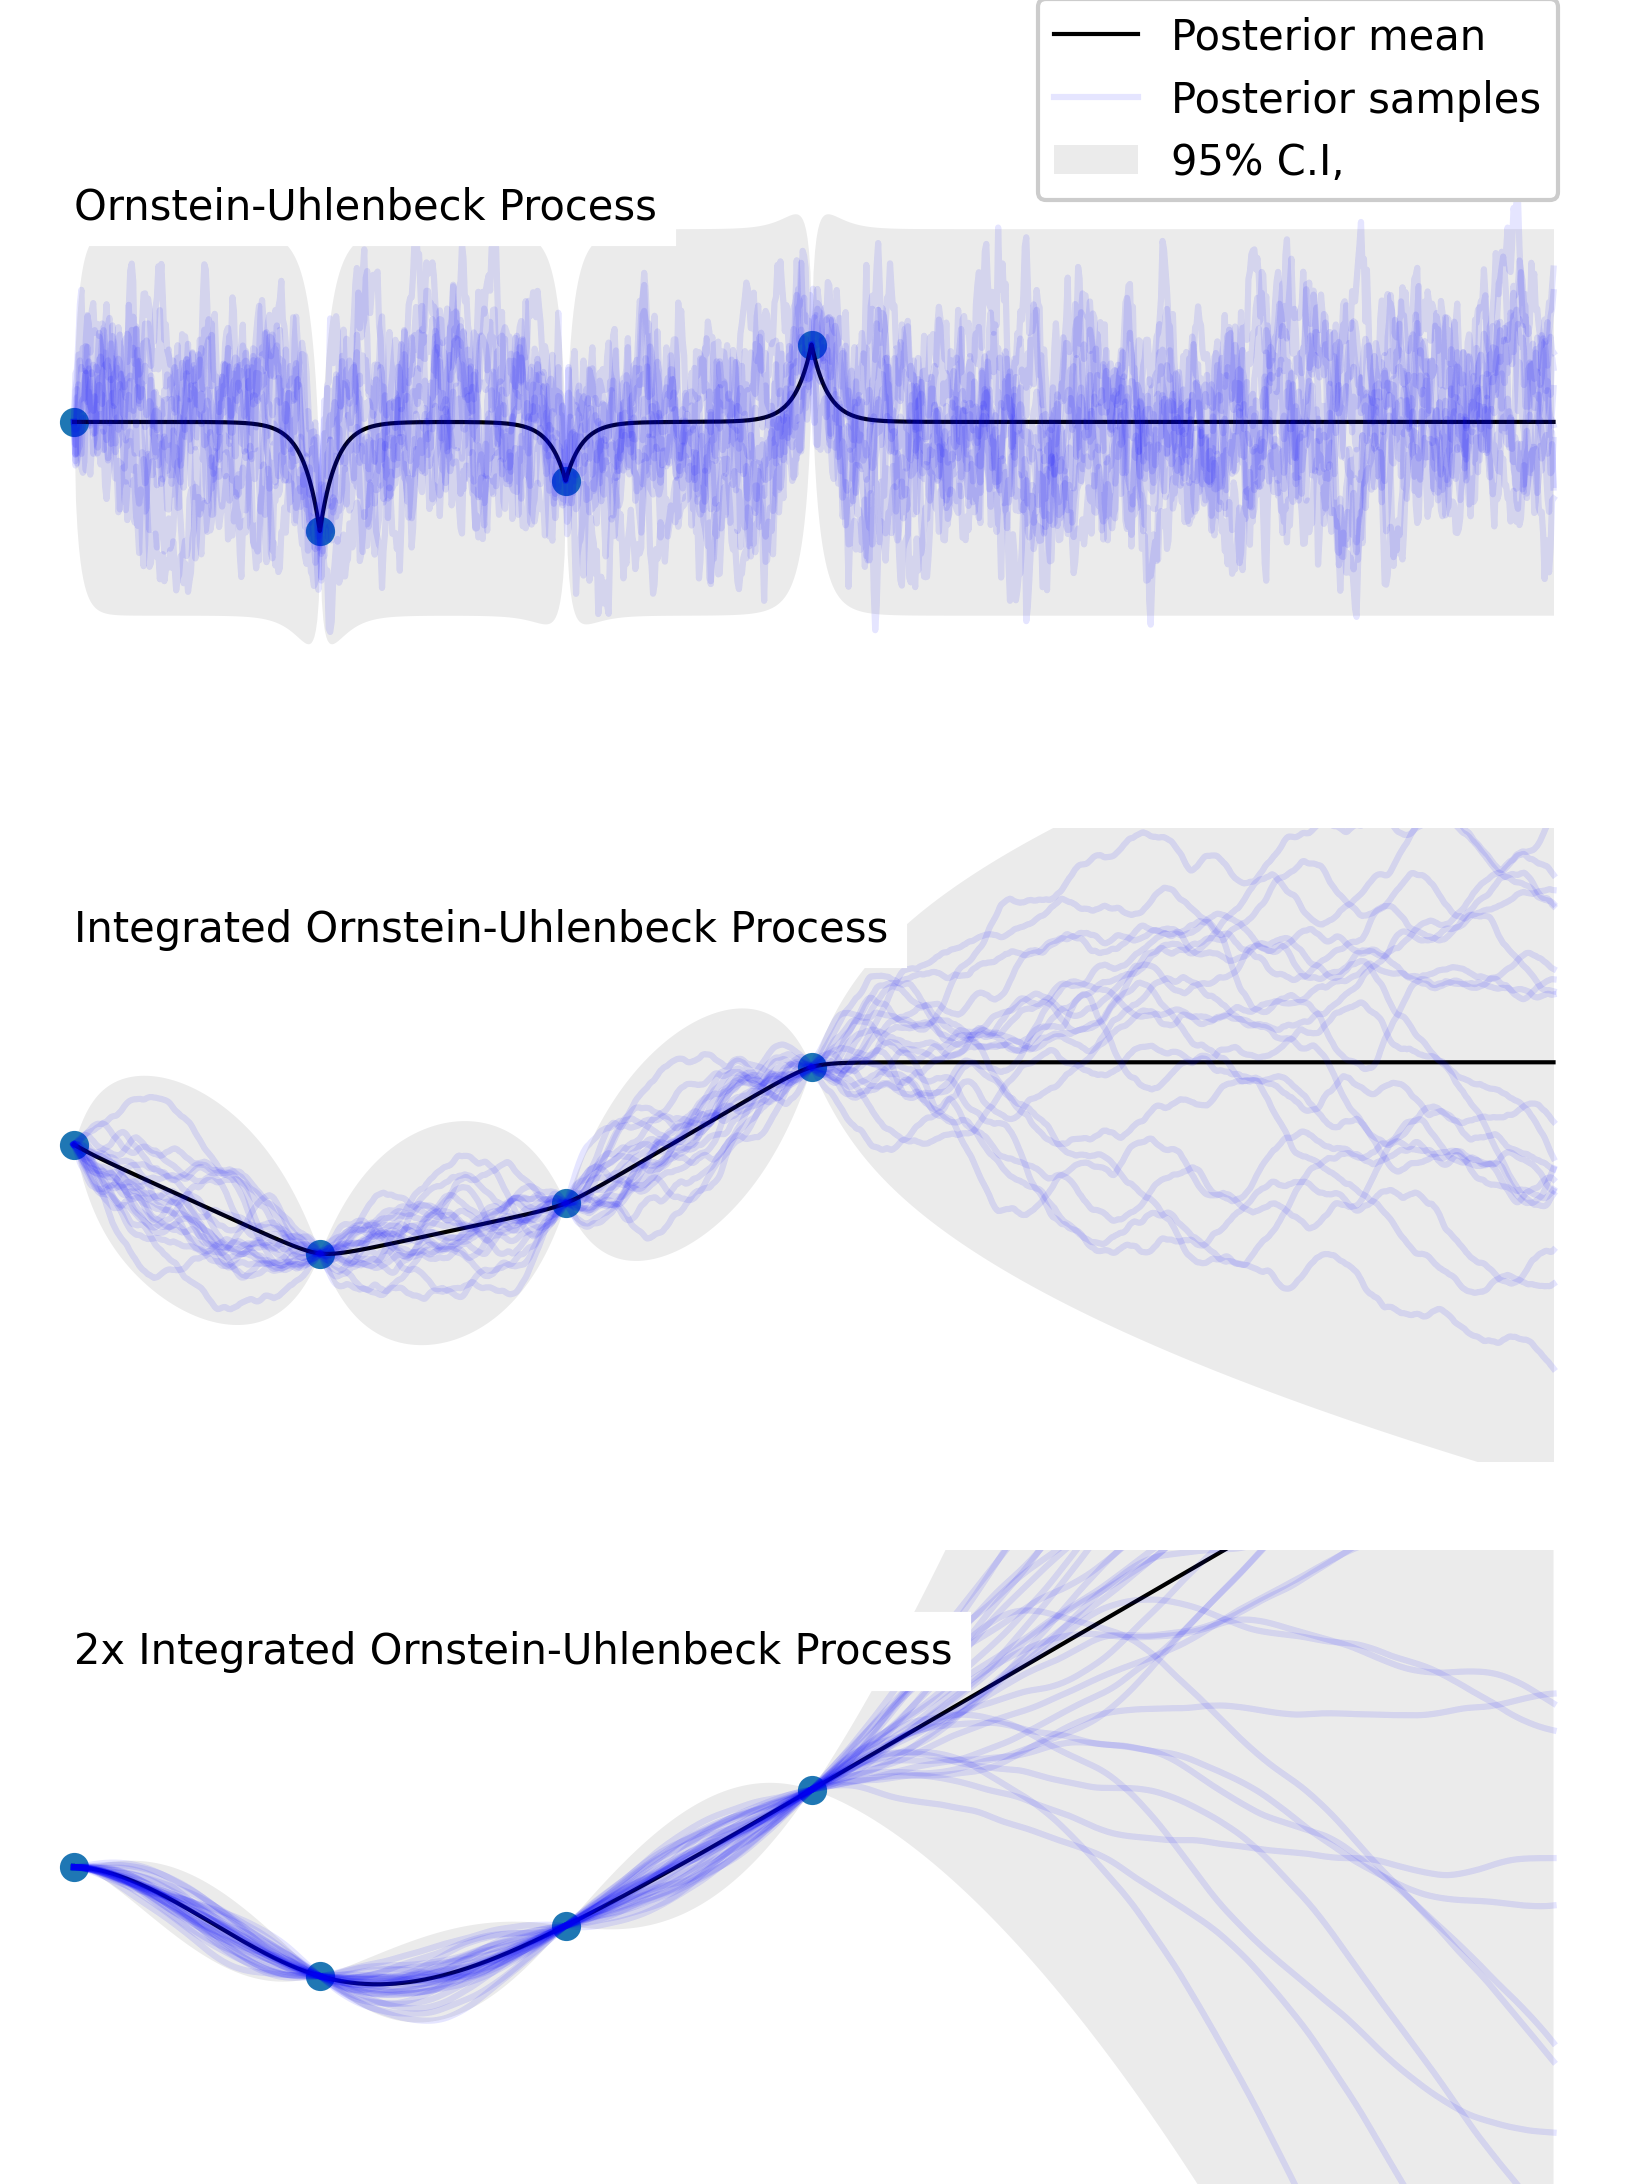
\includegraphics[width=\columnwidth]{../images/conditioned_ous.png}
        \captionof{figure}{Draws from the Integrated Wiener Process, Conditioned}
    \end{center}
    The Ornstein-Uhlenbeck Process depends on rate parameter $a>0$. In terms of eq. \ref{eq:LSDE_definition} its state-space representation is 1-dimensional with $$F=-a  \hspace{1cm}L=1$$ 
    The Integrated Ornstein-Uhlenbeck is the integral of the Ornstein-Uhlenbeck. The state-space representation is 2-dimensional with $$F=\begin{bmatrix}
        0 & 1 \\ 0 & -a
    \end{bmatrix} \hspace{1cm} L=\begin{bmatrix}
        0 & 0 \\ 0 & 1
    \end{bmatrix}$$
    \\ The Twice Integrated Ornstein-Uhlenbeck has 3-dimensional state-space with $$F=\begin{bmatrix}
        0 & 1 & 0 \\ 0 & 0 & 1 \\ 0 & 0 & -a
    \end{bmatrix} \hspace{1cm} L=\begin{bmatrix}
        0 & 0 & 0 \\ 0 & 0 & 0 \\ 0 & 0 & 1
    \end{bmatrix}$$
    In \cite{exponential_probabilistic} they suggest using the Ornstein-Uhlenbeck process to encode prior information to solve particularly difficult "stiff" DEs.\\
    The Ornstein-Uhlenbeck process is mean-reverting (\cite{probnum}), the derivative of the Integrated Ornstein-Uhlenbeck reverts to zero, and the curvature of the Twice Integrated Ornstein-Uhlenbeck reverts to zero.
}
\example{Encoding Prior Dynamics: Wave Process}{
\begin{center}
    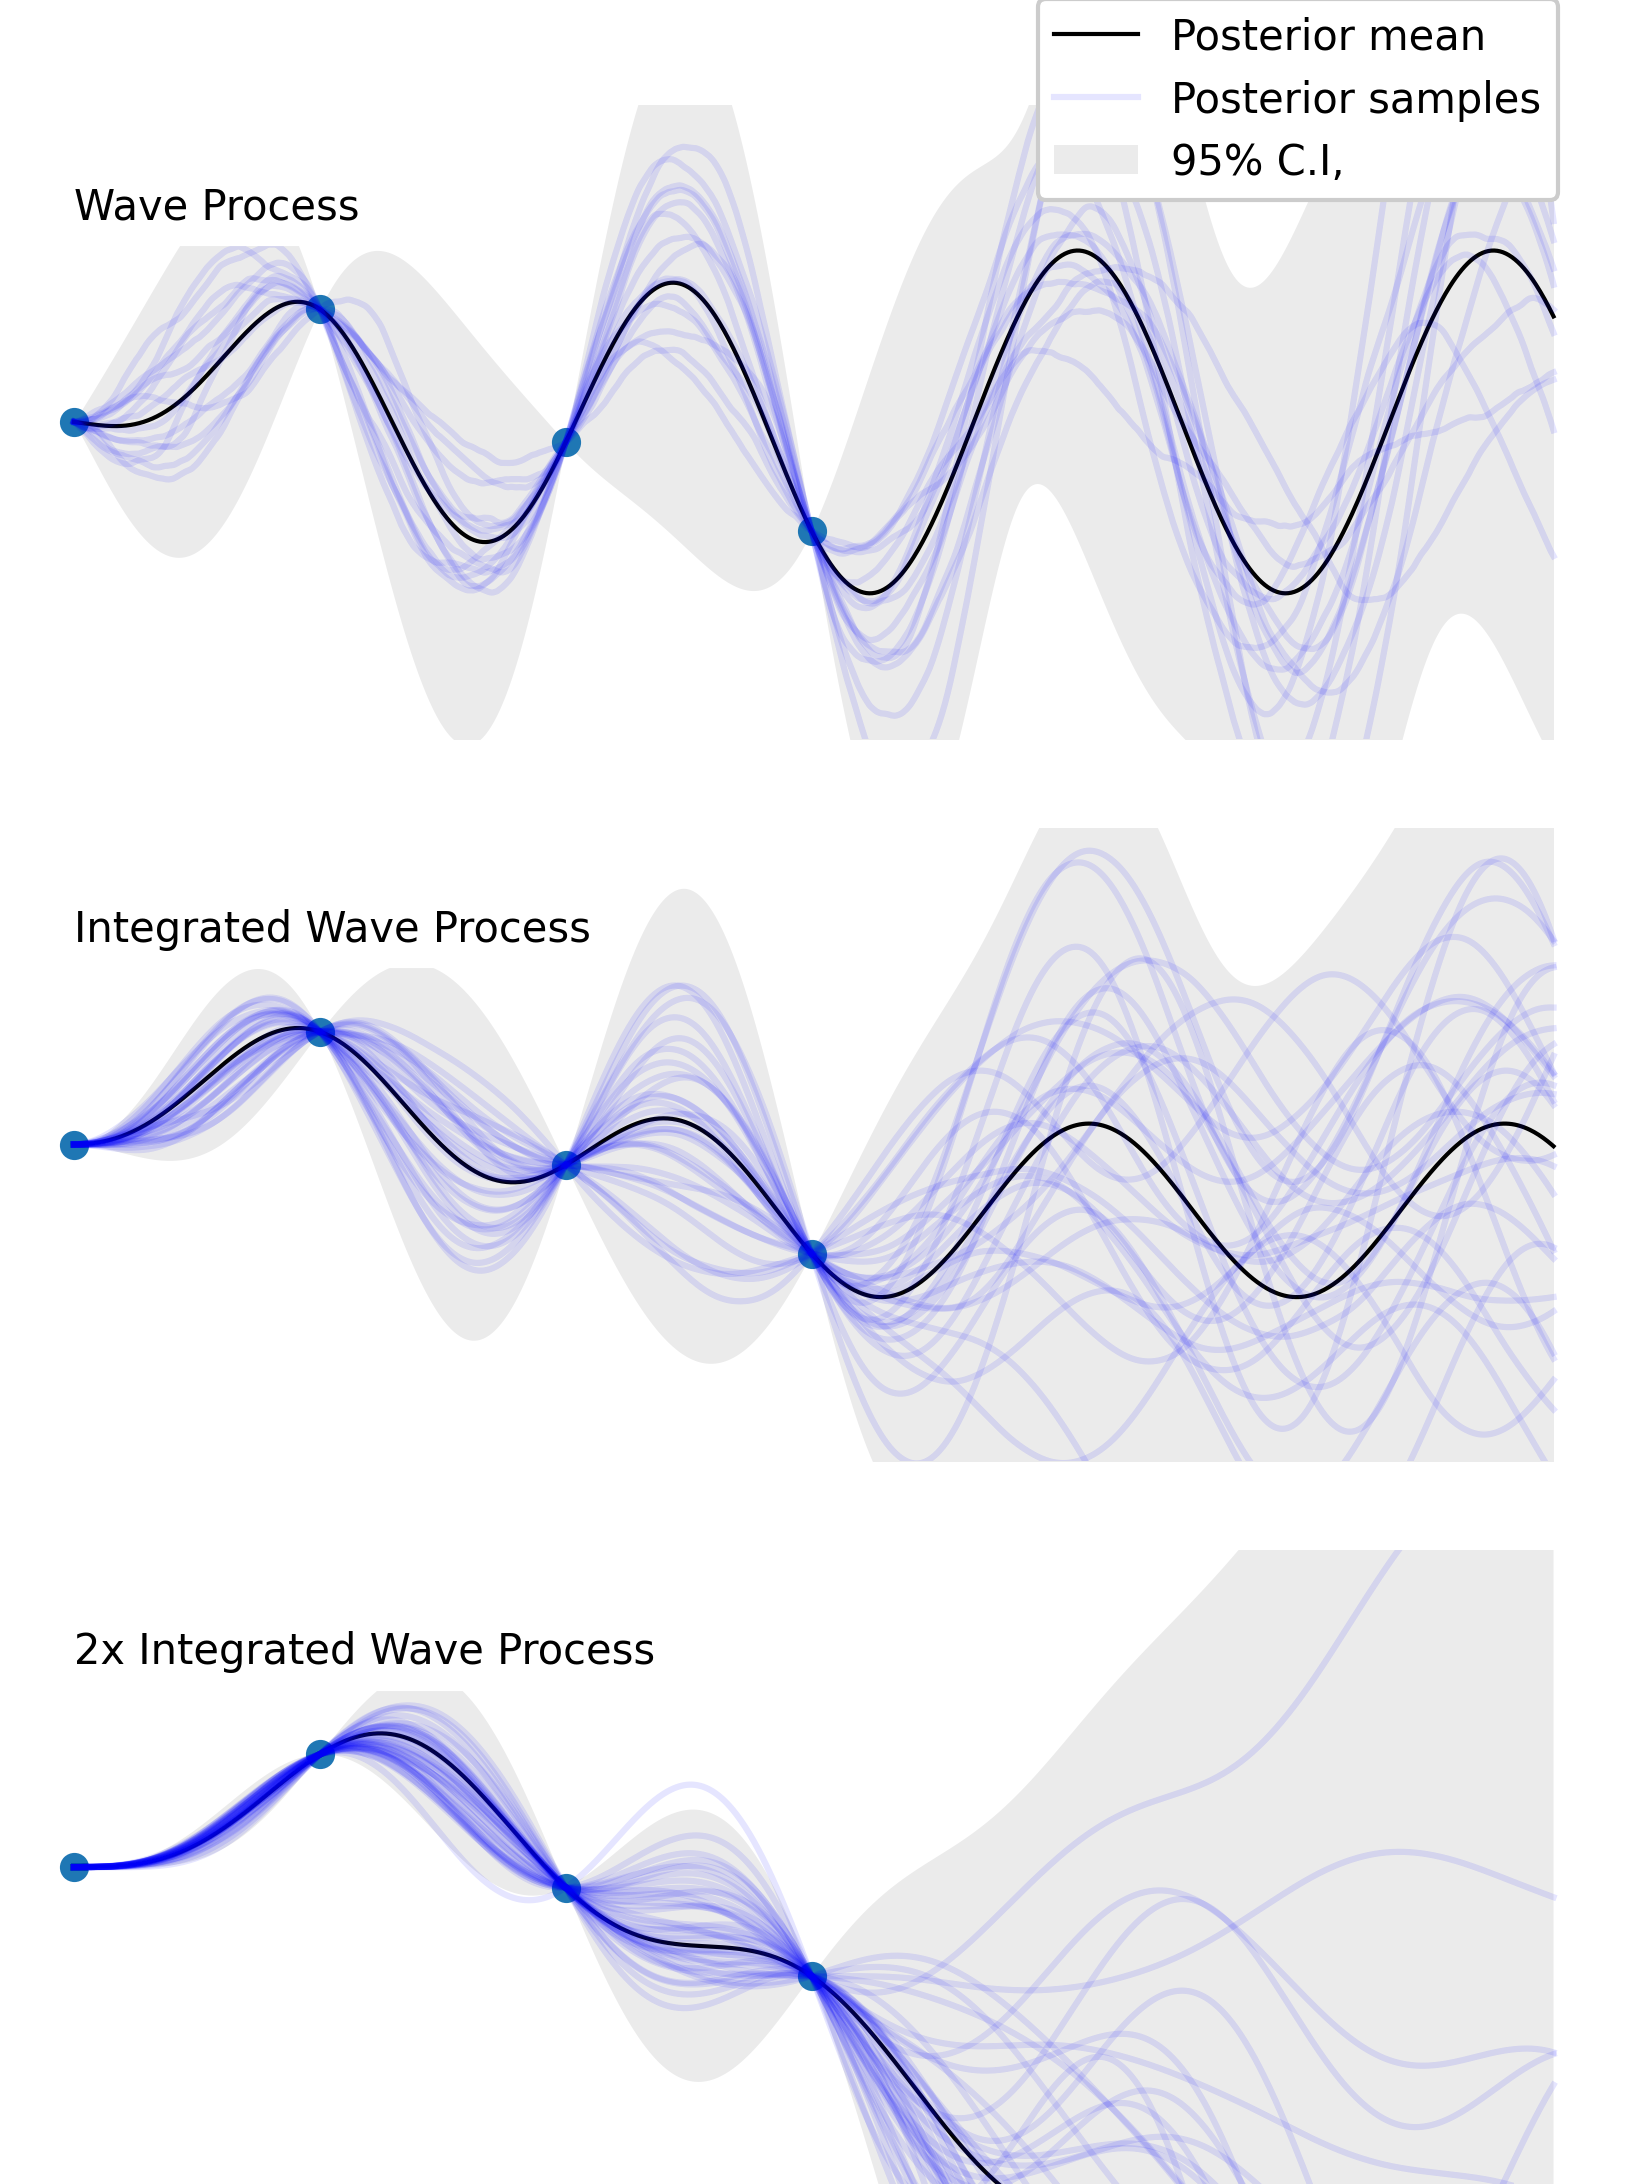
\includegraphics[width=\columnwidth]{../images/conditioned_waves.png}
    \captionof{figure}{Draws from the Integrated Wiener Process, Conditioned}
\end{center}
}


\subsection*{Solving LTI Stochastic Differential Equations}
If the initial distribution is gaussian (which includes a deterministic initial condition) the distribution of a linear SDE can be expresed in closed form. At each time, it will be a multivariate gaussian. For the linear SDE \ref{eq:LSDE_definition}, the following holds
\begin{align}\label{eq:SDE_mean}
    \mathbb{E}[X(t)] = e^{At}\mathbb{E}[X(0)]
\end{align}
Which means, that in expectation the will satisfy the differential equation exactly. This is essentially the same expression as the analytical solution to a deterministic ODE. The covariance matrix of the state at time $t$ is given by
\begin{align}\label{eq:SDE_cov}
    \text{Cov}[X(t)] = \int_0^t e^{A(t-s)}BB^\top e^{A^\top(t-s)} ds
\end{align} TODO CHECK THIS


\subsection*{Discretizing the Prior in Time}
Similarly to the Method Of Lines, we now consider a finite set of times $\mathbb{T} = \{h, 2h, 3h, \dots, T\}$, where $h$ is the timestep size and $T$ is the final time. For simplicity, we choose a fixed timestep, but it can be heterogenous or even adaptive, see \cite{nicoThesis}. 
\\
The Markov property enables the discrete time stochastic recurrence relation (\cite{probnum}) using eq. \ref{eq:SDE_mean} and \ref{eq:SDE_cov}
\begin{align}\label{eq:discrete_time_recurrence}
    \vec{U}(t+h) \;|\; \vec{u}(t) \sim \mathcal{N}(A\vec{u}(t), Q)
\end{align}
with discrete-time transition matrices
\begin{align}
    A &= e^{Fh}\label{eq:easy_matrix_exponential}
    \\
    Q &= \int_0^h e^{Ft}LL^\top e^{F^\top t} dt \label{eq:hard_matrix_exponential}
\end{align}
The formula \ref{eq:easy_matrix_exponential} can be computed numerically quite simply with JAX \cite{jax} or other numerical linear algebra libraries. \ref{eq:hard_matrix_exponential} is however quite difficult, but using Matrix Fraction Decomposition it too can be reduced to a matrix exponential.
\definition{Matrix Fraction Decomposition}{
    The following algorithm for $A$ and $Q$ is originally from \cite{sde-book} but simplified for our fixed-time-step and time-invariant. We will use their notation.
    \\
    Assume the SDE to be discretized is of the form
    $$dX(t) = FX(t)dt + L dW(t)$$ with $F, L \in \reals^{n\times n}$. Compute the matrix exponential of the block-matrix as $M$
    $$M =\exp{\left(h\begin{bmatrix}
        F & L \\ 0 & -F^\top
    \end{bmatrix}\right)}$$
    Extract the upper left block of $M$ as $A\in\reals^{n\times n}$ and the upper right as $C \in \reals^{n\times n}$. Finally, compute $Q$ as $Q = CA^\top$.
}
We can now form the conditional distribution of the state at each time given the state at the previous time. For brevity, we will from here on refer to as the finite-time states $\vec{U}(i\cdot h)$ with an integer subscript index $\vec{U}_i$.When combining the conditonal distribution \ref{eq:discrete_time_recurrence} with an initial gaussian distribution 
$$\vec{U}_0 \sim \mathcal{N}(\mu_0, \Sigma_0)$$ 
we can form the factorized joint distribution of the process across all discrete times as 
$$P(\vec{u}_{\mathbb{T}}) = P(\vec{u}_0, \vec{u}_1, \dots, \vec{u}_{|T|}) =$$
$$\mathcal{N}\Big(\vec{u}_0;\;\mu_0, \Sigma_0\Big)\prod_{t=1}^{|\mathbb{T}|} \mathcal{N}\Big(\vec{u}_t;\;A\vec{u}_{t-1}, Q\Big)$$
This is an instance of a Linear Gaussian Model, which is a tractable and chain-structured bayesian network, depicted below.
\begin{center}
    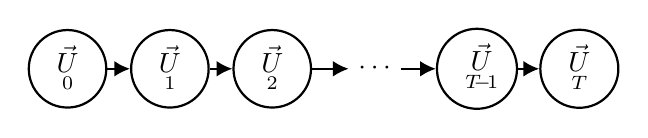
\begin{tikzpicture}[node distance=1.3cm, >={Latex[length=2mm, width=2mm]}, 
        obs/.style={circle, draw, align=center, text width = 3mm, minimum size=3mm, thick, font=\sffamily},
        lat/.style={rectangle, draw, align=center, text width = 6mm, minimum size=6mm, thick, font=\sffamily}]
        
        % Nodes
        \node[obs] (U0) {$\underset{0}{\vec{U}}$};
        \node[obs, right of=U0] (U1) {$\underset{1}{\vec{U}}$};
        \node[obs, right of=U1] (U2) {$\underset{2}{\vec{U}}$};
        \node[right of=U2] (dots) {$\cdots$};
        \node[obs, right of=dots] (UTb) {$\underset{T\!\!-\!1}{\vec{U}}$};
        \node[obs, right of=UTb] (UT) {$\underset{T}{\vec{U}}$};
        
        % Edges
        \draw[->, thick] (U0) -- (U1);
        \draw[->, thick] (U1) -- (U2);
        \draw[->, thick] (U2) -- (dots);
        \draw[->, thick] (dots) -- (UTb);
        \draw[->, thick] (UTb) -- (UT);
    \end{tikzpicture}
\end{center}
The full state of each $\vec{U}_i$ is generally unknown to us, so this joint prior distribution is not by itself of much value to us. To use the joint distribution as a posterior distribution, we need to introduce a likelihood to relate the state to some observations. For this, we describ the idea of the Information Operator (\cite{information_operator}) letting us impose constraints on the state-space representation of the function. For this, the idea of state-projection matrices is useful.
\definition{State Selection Matrices $E_i$}{
    It will be convenient to have an easy way of selecting a specific order derivative $q$ from the state $\vec{U}_i \in \reals^{n\cdot (1+q)}$. We can do so by projecting the full state onto the $q$-th derivative. 
    $$\begin{bmatrix} U \\ \frac{d}{d t} U \\ \cdots \\ \frac{d^q}{d t^q} U\end{bmatrix}$$ We can define the state-projection matrix $E_0$ for the $0$th derivative (the function) as 
    $$E_q = \begin{bmatrix}
        \textbf{I}_n & \textbf{0} & \cdots & \textbf{0}\\
        \textbf{0} & \textbf{0} & \cdots & \textbf{0}\\
        \vdots & \vdots & \ddots & \vdots \\
        \textbf{0} & \textbf{0} & \cdots & \textbf{0}\\
        \end{bmatrix}$$
}
\definition{Information Operator}{
    Although we might not know the complete state at each instant, there might
    We condition on partial observations of some of the time instances (the four blue dots in \ref{fig:iwps}). These optional partial observations can be expressed as $O_i \sim \mathcal{N}(h(\vec{U}_i), \sigma_h)$, where $h$ is a linear function of $\vec{U}_i$.
}
     Each $O_i$ is a function of only the state $\vec{U}_i$, and so the extended Bayesian Network including gaussian Ys takes the following form
    \begin{center}
        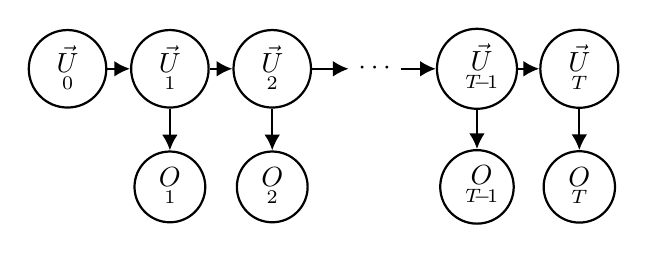
\begin{tikzpicture}[node distance=1.3cm, >={Latex[length=2mm, width=2mm]}, 
            obs/.style={circle, draw, align=center, text width = 3mm, minimum size=3mm, thick, font=\sffamily},
            lat/.style={rectangle, draw, align=center, text width = 6mm, minimum size=6mm, thick, font=\sffamily}]
            
            % Nodes
            \node[obs] (U0) {$\underset{0}{\vec{U}}$};
            \node[obs, right of=U0] (U1) {$\underset{1}{\vec{U}}$};
            \node[obs, right of=U1] (U2) {$\underset{2}{\vec{U}}$};
            \node[right of=U2] (dots) {$\cdots$};
            \node[obs, right of=dots] (UTb) {$\underset{T\!\!-\!1}{\vec{U}}$};
            \node[obs, right of=UTb] (UT) {$\underset{T}{\vec{U}}$};
            
            \node[obs, below of=U1, yshift=-0.2cm] (O1) {$\underset{1}{O}$};
        \node[obs, below of=U2, yshift=-0.2cm] (O2) {$\underset{2}{O}$};
        \node[obs, below of=UTb, yshift=-0.2cm] (OTb) {$\underset{T\!\!-\!1}{O}$};
        \node[obs, below of=UT, yshift=-0.2cm] (OT) {$\underset{T}{O}$};
        
        % Edges
        \draw[->, thick] (U0) -- (U1);
        \draw[->, thick] (U1) -- (U2);
        \draw[->, thick] (U2) -- (dots);
        \draw[->, thick] (dots) -- (UTb);
        \draw[->, thick] (UTb) -- (UT);
        
        \draw[->, thick] (U1) -- (O1);
        \draw[->, thick] (U2) -- (O2);
        \draw[->, thick] (UTb) -- (OTb);
        \draw[->, thick] (UT) -- (OT);    
    \end{tikzpicture}
\end{center}

How did we generate figures \ref{fig:iwps}? We express the factorized joint distribution of the Integrated Wiener Process using Matrix Fraction Decomposition for eqs. \ref{eq:easy_matrix_exponential} and \ref{eq:hard_matrix_exponential}, choose an initial distribution\footnote{The figures use a deterministic initial distribution $\vec{U}(0) \sim \mathcal{N}(\mathbf{0}^n, \mathbf{0}^{n \times n})$}.

The chain-structure of the bayesian network can be exploited to compute the posterior in time $O(|\mathbb{T}|n^3)$(\cite{probnum}) which increases linearly with time. The Kalman-filter and -smoother can be used to compute the full posterior distribution given linear (possibly noisy) transformations $Y_i$ of the state $\vec{U}_i$ at each time.
If one were to form the full joint distribution as one long mean-vector and covariance matrix, the cost of computing the posterior would be of order $O(|\mathbb{T}|^3n^3)$ by the cubic cost of matrix inversion required for the covariance matrix.




\subsection*{Hypothesis: Heat Prior, Wave Prior}
\definition{Heat Prior, Wave Prior}{What is it?}



\ifdefined\COMPILINGFROMMAIN
\else    
    \end{document}
\fi